\chapter{\ifproject%
\ifenglish Experimentation and Results\else การทดลองและผลลัพธ์\fi
\else%
\ifenglish System Evaluation\else การประเมินระบบ\fi
\fi}

\section{การประเมินผลการใช้งาน}
ในส่วนของการประเมินผลการใช้งานแอปพลิเคชันของโครงงานนี้ เราได้แบ่งออกเป็น 2 ประเภท ได้แก่ การทดสอบฝั่ง Flowy (ผู้เช่า) และการทดสอบฝั่ง Flowider (โฮสต์)

\subsection{การทดสอบฝั่ง Flowy}
ทั้งหมด 2 รูปแบบ
\subsubsection{Heuristic Usability Test}
ดังที่กล่าวไว้ว่าโครงงานนี้ให้ความสำคัญกับ User Experience หรือประสบการณ์ของผู้ใช้งานเป็นหลัก เราจึงใช้วิธีการทดสอบแบบ Heuristic Usability Test เพื่อทดสอบและวัดความเข้าใจของผู้ใช้งานตามหลักการ Human-Computer Interaction (HCI)

โดยขั้นตอนวิธีการทดสอบ Heuristic Usability Test มีดังนี้
\begin{enumerate}
    \item เลือกกลุ่มเป้าหมายที่ต้องการใช้งาน Flowy ทั้งหมด 5 คนเป็นผู้ทดสอบ
    \item ให้ผู้ทดสอบใช้งานแอปพลิเคชันตามขั้นตอนหรือขอบเขตการทดสอบแต่ละส่วน โดยไม่มีการอธิบายขั้นตอนการใช้งานล่วงหน้าหรือแม้แต่ระหว่างการใช้งานว่าส่วนใดคืออะไรหรือทำหน้าที่อย่างไร กล่าวคือให้ผู้ทดสอบเผชิญการใช้งานเองทั้งหมดตาม brief
    \item เมื่อสิ้นสุดในแต่ละขอบเขตตาม brief จะให้ผู้ใช้งานลงคะแนนแต่ละส่วนผ่าน Google Form ในแต่ละคำถามเพื่อนำมาสรุปผล
\end{enumerate}
\subsubsection{Problem-Solution Fit}
ดังที่กล่าวไว้ว่าโครงงานนี้ยังให้ความสำคัญกับความสามารถการแข่งขันในเชิงธุรกิจด้วย เราจำใช้วิธีการทดสอบกับกลุ่มลูกค้าเป้าหมาย (customer segment) เพื่อให้รู้แน่ชัดว่าเมื่อผลิตภัณฑ์ของเราออกสู่ตลาดแล้วจะมีลูกค้าเข้ามาใช้บริการของเราอย่างแน่นอน

อย่างไรก็ตามรูปแบบของการทดสอบ Problem-Solution Fit นั้นไม่มีรูปแบบเฉพาะเจาะจงตายตัว ผู้สนใจทดสอบในรูปแบบนี้สามารถออกแบบวิธีการทดสอบด้วยตนเองได้ตามแต่ถนัด

โดยขั้นตอนวิธีการทดสอบ Problem-Solution Fit ในรูปแบบของ Flowy มีดังนี้
\begin{enumerate}
    \item ทำการสุ่มเลือกผู้ทำแบบสอบถามและสนใจจะใช้งาน Flowy (early adopter) ผ่านช่องทาง social media ทั้งหมด 20 คน แล้วติดต่อกลับ
    \item ส่งตัวต้นแบบแอปพลิเคชันของเราให้ early adopter ทั้งหมด 20 คนได้ลองใช้งานและสัมผัสประสบการณ์จำลอง
    \item รอรับความคิดเห็น (feedback) หลังจากใช้งานเสร็จสิ้น
\end{enumerate}

\subsection{การทดสอบฝั่ง Flowider}
ทั้งหมด 1 รูปแบบ
\subsubsection{Phone Interview}
ในส่วนของการทดสอบฝั่ง Flowider ผู้พัฒนาไม่สามารถทดสอบรูปแบบอื่นได้ เนื่องจากปัญหาการพัฒนาแอปพลิเคชันที่ล่าช้า จึงทำให้มีเวลาไม่เพียงพอสำหรับการเจรจาทางธุรกิจกับกลุ่มของ Flowider ซึ่งทำให้ไม่สามารถนำกลุ่ม Flowider เข้าสู่แพลตฟอร์มของเราและทำการทดสอบการใช้งานแอปพลิเคชันได้

อย่างไรก็ตามเราได้ทำการติดต่อผู้ประกอบการหรือเจ้าของพื้นที่ที่มีศักยภาพที่จะเข้ามาอยู่บนแพลตฟอร์มของเราทั้งหมดรวม 10 รายด้วยกัน ซึ่งสามารถแบ่งประเภทได้ดังนี้
\begin{enumerate}
    \item คาเฟ่, ร้านกาแฟ ทั้งหมด 3 ราย
    \item โรงแรม, โฮสเทล ทั้งหมด 4 ราย
    \item สถานที่ส่วนบุคคล, บ้าน, โคเวิร์กกิ้งสเปซ ทั้งหมด 3 ราย
\end{enumerate}

\section{ผลการประเมินการใช้งาน}
\subsection{ผลการทดสอบฝั่ง Flowy}
\textbf{ผลการทดสอบ Heuristic Usability Test}
\begin{figure}[h]
    \begin{center}
    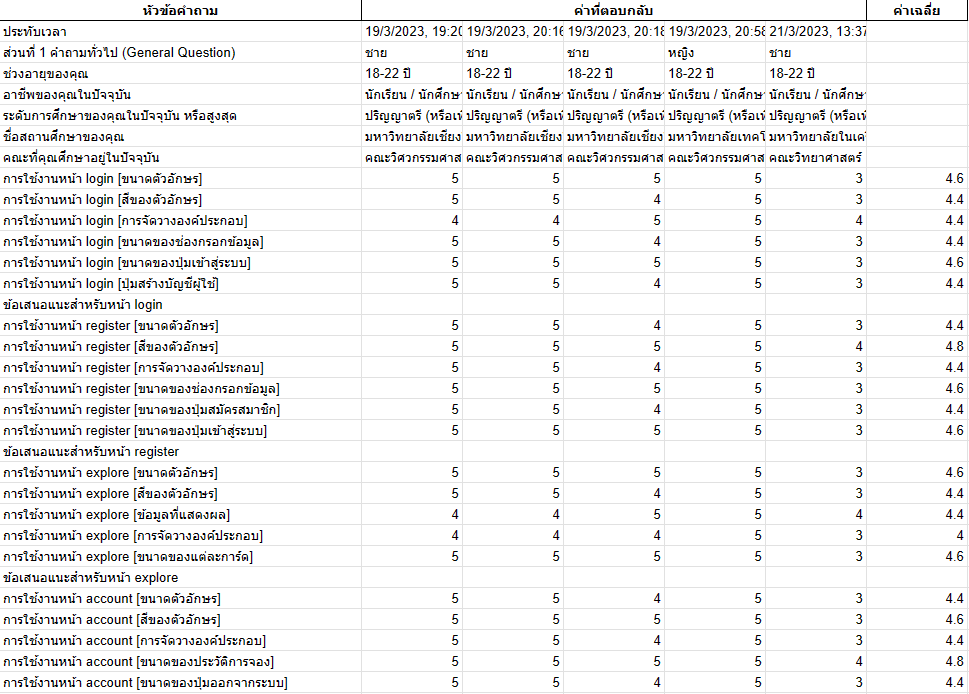
\includegraphics[width=\linewidth]{./image/heuristic_usability_test.png}
    \end{center}
    \caption[Heuristic Usability Test]{รูปภาพผลการทดสอบ Heuristic Usability Test บางส่วน}
    \label{fig:heuristic_usability_test}
\end{figure}

หลังจากได้ทำการทดสอบกับกลุ่มเป้าหมาย 5 คน ผลปรากฎว่า คะแนนเฉลี่ยที่ได้ในแต่ละหัวข้อการทดสอบนั้นอยู่ในช่วง 4 - 4.8 คะแนน ซึ่งสำหรับเกณฑ์ของผู้พัฒนานั้นถือว่าอยู่ในเกณฑ์ที่ดีมาก โดยคะแนนความเข้าใจเฉลี่ยรวมในทุก component ทั้งหมดคือ 4 คะแนนจาก 5 คะแนน และในส่วนของความพึงพอใจจากการใช้งานทั้งหมดคือ 9 คะแนนจาก 10 คะแนน จากช่องตารางสีเขียวดังรูป

\begin{figure}[h]
    \begin{center}
    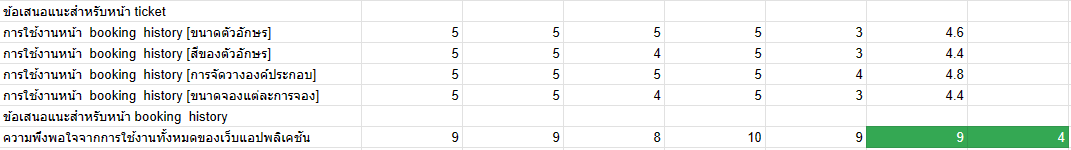
\includegraphics[width=\linewidth]{./image/heuristic_result.png}
    \end{center}
    \caption[Heuristic result]{รูปภาพผลคะแนนการทดสอบเฉลี่ยรวมในช่องตารางสีเขียว}
    \label{fig:heuristic_result}
\end{figure}

จึงสามารถสรุปได้ว่า ณ เวลาที่ได้ทำการทดสอบกับผู้ทดสอบ  User Flow ที่ผู้ใช้งานได้สัมผัสและได้มีประสบการ์ใช้งานจากแอปพลิเคชันของเรา สามารถสื่อสารให้ผู้ใช้งานเข้าใจใน functionality ของส่วนต่าง ๆ ได้เป็นอย่างดี

\subsubsection{ผลการทดสอบ Problem-Solution Fit Test}
จากการทดสอบ Problem-Solution Fit Test กับ early adopter ทั้งหมด 20 คน มีผู้ที่ลงความเห็นว่าจะใช้งาน Flowy แน่นอนหลังจากเปิดตัว public launch ถึง 17 คน ซึ่ง 3 คนที่เหลือที่เลือกจะไม่ใช้งานต่อได้ให้เหตุผลว่า ``อยากให้มีจำนวนของ Flowider มากกว่านี้เพื่อจะได้มีตัวเลือกที่หลากหลายในการเข้าใช้บริการ'' หรือบ้างก็ว่า ``ผลิตภัณฑ์ยังมีความยุ่งยากในการใช้งานมากเกินไปสำหรับตน''
\begin{figure}[h]
    \begin{center}
    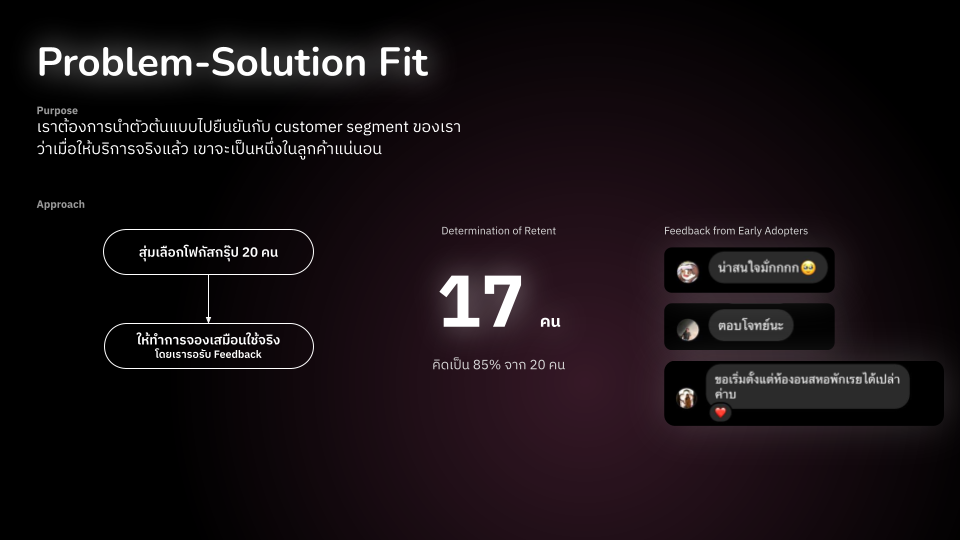
\includegraphics[width=\linewidth]{./image/Problem-Solution_Fit.png}
    \end{center}
    \caption[Problem-Solution Fit]{ผลการทดสอบ Problem-Solution Fit}
    \label{fig:Problem-Solution_Fit}
\end{figure}

\subsection{ผลการทดสอบฝั่ง Flowider}
จากการโทรศัพท์ติดต่อเจรจา มีผู้ประกอบการและเจ้าของพื้นที่สนใจที่จะเป็นส่วนหนึ่งกับแพลตฟอร์มเพียง 3 รายจาก 10 ราย โดยส่วนใหญ่ให้เหตุผลประกอบว่าไม่สะดวกหรือเป็นห่วงเรื่องความปลอดภัยของข้อมูลของผู้ใช้งาน

อย่างไรก็ตามผู้ประกอบการ 3 รายที่มีแนวโน้มจะเข้าร่วมกับแพลตฟอร์ทมของเรานั้นก็มีเงื่อนไขพ่วงในการเข้าร่วมด้วยเช่นกัน โดยต้องการให้ทีมผู้พัฒนาทำจดหมายขออนุญาตอย่างเป็นทางการผ่านภาควิชาวิศวกรรมคอมพิวเตอร์เพื่อขออนุญาตดำเนินการและหาผู้รับผิดชอบหากเกิดเหตุไม่พึงประสงค์ใด ๆ ขึ้น

ทั้งหมดนี้จากข้อจำกัดเรื่องของเวลาที่มีอยู่น้อย ทีมผู้พัฒนาจึงไม่ได้ดำเนินการต่อในช่วงก่อนการนำเสนอการสอบปลายภาค แต่จะดำเนินการต่อหลังจากการสอบปลายภาคเสร็จสิ้นต่อไป
\begin{figure}[h]
    \begin{center}
    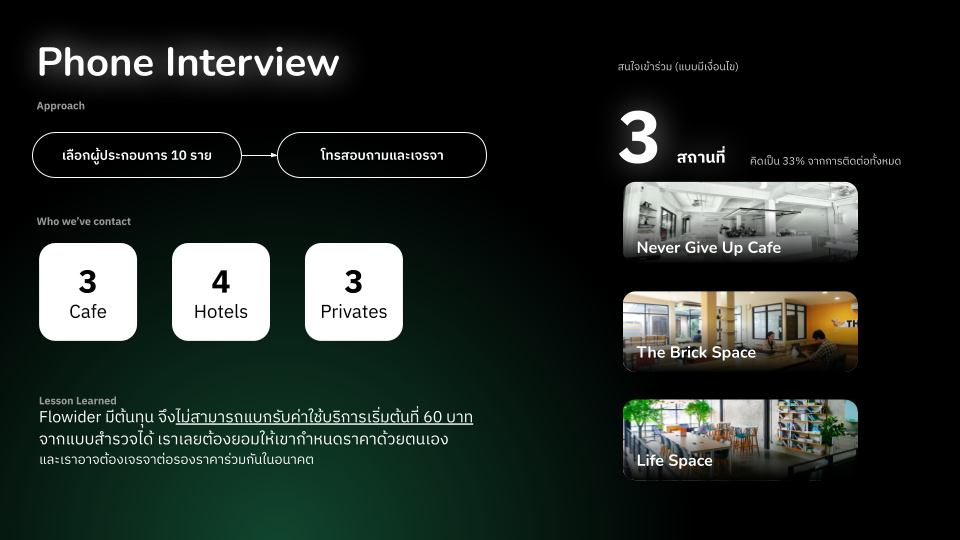
\includegraphics[width=\linewidth]{./image/Phone_interview.png}
    \end{center}
    \caption[Phone Interview]{Phone Interview}
    \label{fig:Phone_interview}
\end{figure}
